\chapter{Fundamentação Teórica}\label{cap:fundamentacao}

Neste capítulo, são apresentados os principais conceitos e definições que fundamentam este trabalho. A \autoref{sec:osteoartrite} aborda a osteoartrite de joelho, destacando suas características clínicas. A \autoref{sec:rnc} introduz as redes neurais convolucionais (RNCs) e as arquiteturas exploradas neste estudo. Em seguida, a \autoref{sec:vision-transformers} apresenta os vision transformers (ViTs) e as arquiteturas escolhidas. A \autoref{sec:funcoes-perda} descreve as funções de perda utilizadas para a comparação entre os modelos. Por fim, a \autoref{sec:avaliacao-metricas} detalha as métricas de avaliação adotadas para comparar o desempenho das diferentes abordagens.

\section{Osteoartrite de Joelho}\label{sec:osteoartrite}

\subsection{Definição e Características Clínicas}

A osteoartrite (OA) é definida como uma doença heterogênea e degenerativa, que afeta as articulações e estruturas ósseas de pacientes, causando dor, deformidade e perda de função \cite{Loeser2012}. Considerando os fenótipos da doença, ou seja, as características clínicas e radiográficas observáveis, a OA é considerada altamente heterogênea e pode ser desencadeada por diferentes fatores de risco, entre os quais destacam-se idade avançada, sexo (maior prevalência em mulheres, sobretudo após a menopausa), obesidade (que aumenta a carga mecânica nas articulações) e predisposição genética \cite{ShaneAnderson2010, Tschon2021, PACCA2018, Spector2004}. Outros fatores, como histórico de lesões articulares, atividade física intensa e doenças metabólicas, também podem contribuir para o desenvolvimento da doença.

A OA pode afetar diversas articulações, como joelhos, quadris, mãos, ombros, entre outras. No entanto, a junção do joelho é a área mais afetada devido ao suporte do peso corporal que está diretamente associado a movimentos essenciais, como caminhar, subir escadas e agachar \cite{Kanamoto2020}. Portanto, tais fatores fazem com que a doença seja uma das principais causas de dor crônica e incapacidade funcional, levando a uma necessidade de identificar e classificar a OA de forma precisa e precoce, para que o tratamento seja iniciado o mais cedo possível a fim de retardar a progressão da doença e melhorar a qualidade de vida dos pacientes.

\subsection{Mudanças Patológicas da OA de Joelho}

As alterações patológicas observadas na osteoartrite de joelho afetam diferentes estruturas articulares e podem ser identificadas por exames de imagem, como a ressonância magnética. A \autoref{fig:osteoartrite-joelho} ilustra essas mudanças.

Inicialmente, observa-se a inflamação sinovial, ou sinovite, representada na imagem (A) pela área destacada pela seta branca espessa. A membrana sinovial inflamada passa a liberar mediadores inflamatórios que contribuem para a destruição da cartilagem articular \cite{Pessler2008}.  

Na sequência, alterações do osso subcondral tornam-se evidentes, como a formação de cistos (B, seta branca) e o edema da medula óssea (C, setas brancas finas). Tais processos estão associados ao aumento da carga mecânica e ao remodelamento ósseo anormal \cite{vanderKraan2007}.  

A degradação da cartilagem articular, característica central da OA, é mostrada em (D–F). O desgaste pode ser parcial (D, seta preta espessa) ou total (E–F, setas pretas finas), comprometendo a função de absorção de impactos e resultando em atrito ósseo. Esse processo é impulsionado pela ativação dos condrócitos, que aumentam a produção de enzimas degradativas \cite{Goldring2009}.  

Associadas a essas alterações, observam-se a esclerose subcondral (E–F, cabeça de seta) e a formação de osteófitos marginais (E–F, seta dupla), que refletem o remodelamento ósseo compensatório, mas acabam restringindo a mobilidade articular e causando dor. Além disso, a degeneração dos meniscos e ligamentos, embora não esteja diretamente ilustrada na figura, também contribui para a perda da estabilidade articular e para a progressão da doença \cite{Loeser2012}.  

\begin{figure}[!htbp]
    \centering
    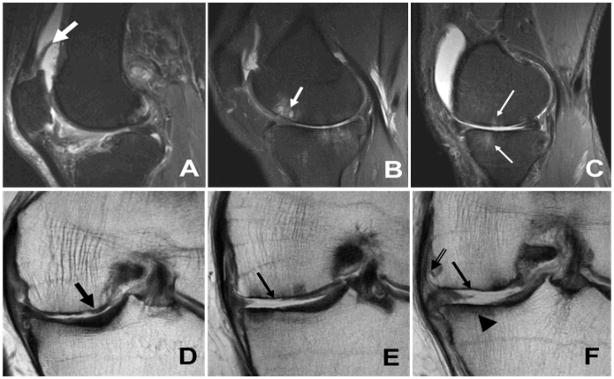
\includegraphics[width=\linewidth]{figs/mud-patologicas-oa.jpg}
    \caption{Imagens de ressonância magnética na osteoartrite de joelho. (A) Sinovite reativa (seta branca espessa), (B) Formação de cistos subcondrais (seta branca), (C) Edema da medula óssea (setas brancas finas), (D) Desgaste parcial da cartilagem (seta preta espessa), (E–F) Desgaste total da cartilagem (setas pretas finas), esclerose subcondral (cabeça de seta) e osteófitos marginais (seta dupla). Fonte: \citeonline{Loeser2012}.}
    \label{fig:osteoartrite-joelho}
\end{figure}

\subsection{Impacto da OA na Qualidade de Vida}

De acordo com a \textit{World Health Organization} (WHO), a expressão ``qualidade de vida'' é entendida como a percepção que o indivíduo possui sobre sua posição na vida. Essa avaliação é feita dentro do contexto da cultura e do sistema de valores em que está inserido, considerando ainda seus objetivos, expectativas, padrões e preocupações \cite{who2012}.

Existe um grande esforço de pesquisadores e especialistas para avaliar o grau de incapacidade física causado pela doença, além de avaliar os efeitos de diferentes tratamentos em aspectos como dor, função física e mobilidade. No entanto, tais manifestações físicas afetam diretamente outras áreas na vida dos pacientes, como interações sociais, saúde mental e qualidade do sono \cite{Ferrel1992}. Em comparação com outras doenças crônicas, pacientes com doenças muscoesqueléticas, como a OA, são os mais afetados em termos de qualidade de vida. A OA de joelho, especificamente, tende a declinar progressivamente a qualidade de vida conforme a progressão da doença \cite{Hoogeboom2013}.

\citeonline{Desmeules2009} realizaram um estudo com 197 pacientes com cirurgia agendada para substituição total do joelho (\textit{Total Knee Arthroplasty} - TKA) e avaliaram, através da escala de qualidade de vida SF-36 \cite{Ware1992}, a relação entre a OA de joelho e a qualidade de vida. Os resultados mostraram que a pontuação média da qualidade de vida dos pacientes era significativamente menor do que a população geral no Canadá ($p < 0,05$). Outros estudos também mostraram resultados similares em pacientes esperando por TKA \cite{Snider2005,Kapetanakis2011}. É razoável, portanto, que pacientes com OA de joelho severa tenham baixos níveis de qualidade de vida comparado com a população geral.

\citeonline{Sutbeyaz2007} fizeram um estudo com 28 pacientes obesos com OA de joelho e também avaliaram a qualidade de vida através da escala SF-36. Os resultados mostraram que os pacientes obesos tiveram pontuações muito mais baixas em todos os domínios da escala SF-36, em comparação com o grupo de controle ($p < 0,001$). Com isso, a obesidade foi associada a uma pior qualidade de vida em pacientes com OA de joelho, o que sugere que a perda de peso pode ser benéfica para melhorar o panorama desses pacientes.

Complementarmente, \citeonline{Kawano2015} mostraram que existe uma relação do nível de escolaridade com a capacidade funcional e dor em pacientes com OA de joelho. O estudo foi conduzido com 93 pacientes tratados no Serviço de Ortopedia e Traumatologia do Hospital Santa Izabel e Santa Casa da Misericórdia da Bahia, em Salvador, Brasil. A avaliação da qualidade de vida foi feita através do questionário SF-36 e mostrou que pacientes com níveis mais baixos de escolaridade tiveram pontuações mais baixas nos domínios de capacidade funcional ($p < 0,001$), limitação funcional ($p = 0,009$) e dor ($p = 0,01$), em comparação com pacientes com níveis mais altos de escolaridade ($p < 0,05$). Com isso, a escolaridade foi associada a uma melhor qualidade de vida em pacientes com OA de joelho, o que sugere que a educação também pode ser um fator importante nesse cenário.

\subsection{Prevalência da OA}

Dados recentes do \textit{Global Burden of Disease} (GBD) — o estudo epidemiológico observacional mais abrangente do mundo — revelaram que a prevalência da OA cresceu 132\% entre 1990 e 2020, com projeções de crescimento de 60 a 100\% até 2050, alcançando a marca de 1 bilhão de pessoas. Com uma prevalência de 7,6\% da população global em 2020, o que equivale a aproximadamente 595 milhões de pessoas, a OA é mais comum em países desenvolvidos, devido à correlação com o status socieconômico, e contribui significativamente para os chamados ``anos vividos com incapacidade'' (\textit{Years Lived with Disability} - YLD). Além disso, o estudo também aponta que a OA é mais comum em mulheres do que em homens, com prevalência de 8,0\% e 5,8\%, respectivamente, além de atingir principalmente idosos, especialmente aqueles acima de 70 anos, onde a OA assume a 7ª posição entre as principais causas de incapacidade, primeiramente afetando a articulação do joelho \cite{COURTIES20241397}.

No Brasil, \citeonline{RodriguesSenna2004} realizaram um estudo com mais de 3 mil pessoas e identificaram cerca de 7,2\% com doenças reumáticas, sendo a OA a mais comum, com prevalência de 4,14\%. Essa prevalência tende a aumentar visto que, além de existir uma correlação entre a OA e a obesidade, estima-se que o Brasil tenha uma taxa de sobrepeso e obesidade combinados de 68,1\% em 2030 \cite{fiocruz2024}.

\subsection{Diagnóstico e Métodos de Avaliação da OA}

O diagnóstico da OA normalmente é feito com base em exames clínicos, como a avaliação dos sintomas do paciente, exames de imagem, como radiografias e ressonâncias magnéticas, e exames laboratoriais, como a análise do líquido sinovial \cite{Kraus2015}. Exames de raio-x têm sido o método mais comum para diagnosticar a OA, pois é uma abordagem acessível que permite visualizar o espaço articular, além de alterações ósseas e cartilaginosas nas articulações, como a formação de osteófitos.

Essa avaliação é tipicamente feita por radiologistas a partir de radiografias do joelho extendido ou flexionado, dependendo da necessidade de visualização intra-articular \cite{Braun2012}. A partir dessas imagens, é possível fazer a classificação da severidade da OA e, em caso de diagnóstico, recomendar tratamentos farmacêuticos e não farmacêuticos, como exercícios de fortalecimento muscular e fisioterapia.

\subsection{Classificação da OA}

A classificação radiográfica da osteoartrite foi proposta por \citeonline{KELLGREN1957}, que desenvolveram a escala de Kellgren/Lawrence (KL). Essa escala considera principalmente a presença de osteófitos, o estreitamento do espaço articular e a esclerose subcondral, permitindo graduar a progressão da doença em cinco estágios: 0 (saudável), 1 (duvidoso), 2 (mínimo), 3 (moderado) e 4 (grave), conforme ilustrado na \autoref{tabela-kl}.  

Na prática clínica, a atribuição do grau KL é realizada por radiologistas, que analisam as radiografias de acordo com sua experiência e julgamento clínico. Entretanto, esse processo é inerentemente subjetivo e suscetível a variações entre avaliadores, podendo resultar em diagnósticos tardios ou inconsistentes. Tal limitação reforça a importância de métodos complementares que busquem maior padronização e precisão, sobretudo em contextos onde a detecção precoce é crucial para retardar a progressão da doença.

\begin{table}[h]
    \centering
    \caption{Escala de Kellgren/Lawrence para classificação da severidade de osteoartrite.}
    \label{tabela-kl}
    \begin{tabular}{|c|c|c|c|c|}
        \hline
        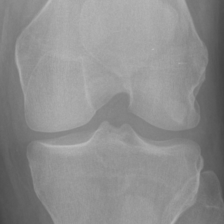
\includegraphics[width=1.7cm]{figs/KL0-sample.png} & 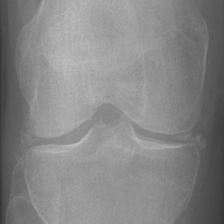
\includegraphics[width=1.7cm]{figs/KL1-sample.png} & 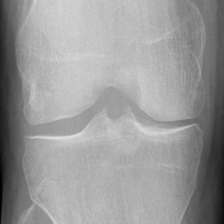
\includegraphics[width=1.7cm]{figs/KL2-sample.png} & 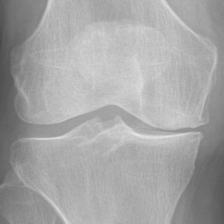
\includegraphics[width=1.7cm]{figs/KL3-sample.png} & 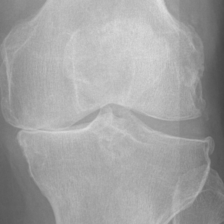
\includegraphics[width=1.7cm]{figs/KL4-sample.png} \\
        \hline
        \textbf{0 (saudável)} & \textbf{1 (duvidoso)} & \textbf{2 (mínimo)} & \textbf{3 (moderado)} & \textbf{4 (severo)} \\
        \hline
    \end{tabular}
\end{table}

\section{Rede Neural Convolucional (RNC)}\label{sec:rnc}

Uma rede neural artificial é um modelo computacional inspirado no cérebro humano \cite{McCulloch1943}, onde neurônios artificiais recebem um conjunto de entradas ponderadas, realizam uma soma dessas entradas e aplicam uma função de ativação para produzir uma saída. Essa estrutura permite que as redes neurais aprendam padrões complexos a partir de dados, tornando-as adequadas para tarefas de processamento de linguagem natural, visão computacional, entre outras aplicações.

Em 2006, \citeonline{Hinton2006} propuseram o uso de redes neurais artificiais com múltiplas camadas com o objetivo de melhorar a capacidade dos modelos, o que levou a um renascimento do interesse nessas redes e ao desenvolvimento de novas arquiteturas, como é o caso da rede neural convolucional (RNC). As RNCs são modelos de aprendizado profundo projetados para processar dados com estrutura de grade, como imagens. Inspiradas na organização do córtex visual, RNCs são amplamente utilizadas em tarefas de visão computacional, como classificação de imagens, detecção de objetos e segmentação semântica.

A camada de convolução é o componente central das RNCs, responsável por extrair características locais dos dados de entrada. Essa camada utiliza filtros, que são pequenas matrizes de pesos (por exemplo, 3×3 ou 5×5) aplicadas em toda a imagem de entrada para gerar um mapa de características, representando a presença dessas características em diferentes regiões da imagem.

Esses filtros são ajustados durante o treinamento da rede, permitindo que a RNC aprenda a detectar padrões relevantes, como bordas, texturas e formas. Conforme a rede avança pelas camadas, os filtros se tornam mais complexos e capazes de capturar características de alto nível, como objetos inteiros. Após as convoluções, é comum utilizar a função de ativação \textit{Rectified Linear Unit} (ReLU), que substitui valores negativos por zero e introduz não linearidades no modelo, permitindo que ele aprenda representações complexas.

Após as camadas de convolução, as RNCs geralmente incluem camadas de \textit{pooling} para reduzir a dimensionalidade dos mapas de características, enquanto preservam as características mais relevantes. O \textit{pooling} pode ser feito de várias maneiras, como \textit{max pooling} (onde o valor máximo de uma região é mantido) ou \textit{average pooling} (onde a média dos valores é calculada). Esse processo contribui para reduzir a quantidade de parâmetros e o custo computacional da rede, além de tornar a rede mais robusta a pequenas variações nos dados de entrada.

Após diversas camadas de convolução e \textit{pooling}, uma ou mais camadas totalmente conectadas são adicionadas ao final da rede para combinar as características extraídas de camadas anteriores e realizar a tarefa de classificação. Cada neurônio dessas camadas está conectado a todos os neurônios da camada anterior, permitindo decisões baseadas em combinações globais das informações aprendidas. Em tarefas de classificação, essa camada geralmente utiliza a função de ativação \textit{softmax}, que transforma as saídas em probabilidades.

Durante o treinamento, a RNC ajusta os pesos dos filtros por meio do algoritmo de retropropagação, em que o erro de saída é retropropagado pela rede para atualizar os pesos e minimizar a função de perda. Esse processo é repetido por várias épocas, permitindo que a rede aprenda a reconhecer padrões complexos nos dados de entrada.

A \autoref{fig:cnn} ilustra uma rede neural convolucional composta por cinco camadas. O número de camadas, a disposição dessas camadas, o número e tamanho dos filtros, a forma de conexão entre as camadas, entre outros fatores, podem variar dependendo da arquitetura escolhida. Em seguida, serão apresentadas algumas das arquiteturas populares de RNC que foram utilizadas neste trabalho.

\begin{figure}[!htbp]
    \centering
    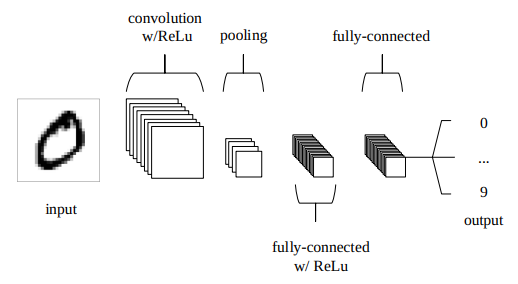
\includegraphics[width=0.7\linewidth]{figs/convolution-neural-network.png}
    \caption{Uma rede neural convolucional simples, composta por apenas cinco camadas. Fonte: \citeonline{Saxena2022}.}
    \label{fig:cnn}
\end{figure}

\subsection{Visual Geometry Group Network (VGG)}

Os modelos VGG foram introduzidos pelo \textit{Visual Geometry Group} da Universidade de Oxford por \citeonline{Simonyan2015}, que depois serviu como base para a competição do ImageNet em 2014, quando conquistaram o primeiro e segundo lugar na época. A arquitetura VGG é conhecida por sua simplicidade e profundidade, utilizando filtros convolucionais pequenos (3×3) empilhados em camadas profundas, variando de 11 a 19 camadas. O objetivo dos autores era explorar o impacto da profundidade na performance do modelo, e eles descobriram que redes neurais mais profundas superavam redes mais rasas, desde que treinadas adequadamente.

A arquitetura VGG processa imagens RGB de 224×224 pixels, utilizando uma série de camadas convolucionais seguidas por camadas de \textit{pooling}, onde cada camada contém um número crescente de filtros 3×3. O \textit{stride} é fixo em 1 pixel, e o \textit{padding} é utilizado para manter a dimensão da imagem. Após as camadas convolucionais, são aplicadas camadas de \textit{max-pooling} com um tamanho de 2×2 e \textit{stride} de 2, reduzindo a dimensão da imagem pela metade. Por fim, são adicionadas três camadas totalmente conectadas, seguidas por uma camada de saída com ativação \textit{softmax} para classificação. Além disso, as camadas ocultas são ativadas por funções ReLU, responsáveis por introduzir a não-linearidade no modelo.

A \autoref{tab:vgg-arch} apresenta a configuração das arquiteturas VGG-16 e VGG-19, com um total de 16 e 19 camadas, respectivamente. Ambas se destacaram na competição do ImageNet e são amplamente utilizadas devido à sua performance em tarefas de classificação, incluindo o diagnóstico a partir de imagens médicas \cite{Saini2023, Sitaula2021}.

\begin{table}[!htbp]
    \centering
    \caption{Configuração dos modelos VGG-16 e VGG-19. Fonte: \citeonline{Simonyan2015}.}
    \label{tab:vgg-arch}
    \footnotesize
    \begin{tabular}{|c|c|}
        \hline
        \textbf{VGG-16} & \textbf{VGG-19} \\
        \hline
        16 camadas & 19 camadas \\
        \hline
        \multicolumn{2}{|c|}{imagem RGB de entrada (224 x 224)} \\
        \hline
        conv3-64 & conv3-64 \\
        conv3-64 & conv3-64 \\
        \hline
        \multicolumn{2}{|c|}{maxpool} \\
        \hline
        conv3-128 & conv3-128 \\
        conv3-128 & conv3-128 \\
        \hline
        \multicolumn{2}{|c|}{maxpool} \\
        \hline
        conv3-256 & conv3-256 \\
        conv3-256 & conv3-256 \\
        conv3-256 & conv3-256 \\
         & \textbf{conv3-256} \\
        \hline
        \multicolumn{2}{|c|}{maxpool} \\
        \hline
        conv3-512 & conv3-512 \\
        conv3-512 & conv3-512 \\
        conv3-512 & conv3-512 \\
         & \textbf{conv3-512} \\
        \hline
        \multicolumn{2}{|c|}{maxpool} \\
        \hline
        conv3-512 & conv3-512 \\
        conv3-512 & conv3-512 \\
        conv3-512 & conv3-512 \\
         & \textbf{conv3-512} \\
        \hline
        \multicolumn{2}{|c|}{maxpool} \\
        \hline
        \multicolumn{2}{|c|}{FC-4096} \\
        \hline
        \multicolumn{2}{|c|}{FC-4096} \\
        \hline
        \multicolumn{2}{|c|}{FC-1000} \\
        \hline
        \multicolumn{2}{|c|}{softmax} \\
        \hline
    \end{tabular}
\end{table}

\subsection{Residual Network (ResNet)}

\citeonline{He2016} venceram a competição ILSVRC 2015 com a arquitetura ResNet, que introduziu a ideia de blocos residuais e alcançou uma taxa de erro de 3,57\% no conjunto de validação do ImageNet com um \textit{ensemble} de seus modelos. Os autores abordaram o problema da degradação de desempenho: conforme a profundidade da rede aumentava, a acurácia saturava e começava a diminuir. Para resolver, eles introduziram a ideia de conexões de atalho entre as camadas, onde o sinal de entrada de uma camada é somado ao sinal de saída de uma camada subsequente (\autoref{fig:residual-learning}).

\begin{figure}[!htbp]
    \centering
    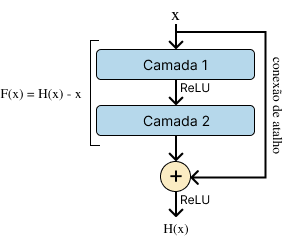
\includegraphics[width=0.5\linewidth]{figs/residual-connection.png}
    \caption{Aprendizado residual introduzido pela arquitetura ResNet.}
    \label{fig:residual-learning}
\end{figure}

Formalmente, considerando que o objetivo de uma rede neural é aprender uma função \( H(x) \), onde \( x \) é a entrada, a ResNet propõe que a rede aprenda uma função residual \( F(x) = H(x) - x \), onde a entrada \( x \) é adicionada à saída \( H(x) \), reformulando a função de aprendizado como \( H(x) = F(x) + x \). Essa abordagem permite que a rede aprenda funções de identidade mais facilmente, facilitando o treinamento de redes mais profundas sem adicionar complexidade.

A arquitetura ResNet é composta por pilhas de blocos residuais que consistem em duas camadas convolucionais, com uma normalização em lote e uma função de ativação ReLU entre elas. As camadas convolucionais utilizam filtros de tamanho 3×3, com um \textit{stride} de 1 e \textit{padding} de 1, para manter a dimensão da imagem. A saída do bloco residual é então somada à entrada original, permitindo que o modelo aprenda a função residual. A rede termina com uma camada de \textit{average pooling} global e uma camada totalmente conectada com ativação \textit{softmax} para classificação.

A \autoref{resnet-arch} apresenta a configuração das arquiteturas ResNet-34, ResNet-50 e ResNet-101, que são variantes da ResNet com diferentes profundidades. Essas arquiteturas são amplamente utilizadas devido à sua eficácia em tarefas de classificação de imagens, especialmente em radiografias. Como exemplo, \citeonline{Leung2020} utilizaram a arquitetura ResNet-34 para diagnosticar a OA de joelho em pacientes submetidos à TKA e obtiveram resultados que superaram modelos de resultados binários.

\begin{table}[!htbp]
    \centering
    \caption{Configuração dos modelos ResNet-34, ResNet-50 e ResNet-101. Fonte: \citeonline{He2016}.}
    \label{resnet-arch}
    \footnotesize
    \begin{tabular}{|c|c|c|c|c|}
        \hline
        \textbf{Camada} & \textbf{Tamanho da saída} & \textbf{34 camadas} & \textbf{50 camadas} & \textbf{101 camadas} \\
        \hline
        conv1 & 112×112 & \multicolumn{3}{c|}{7×7, 64, stride 2} \\
        \hline
        \multicolumn{2}{|c|}{ } & \multicolumn{3}{c|}{3×3 max pool, stride 2} \\
        \hline
        conv2\_x & 56×56 & 
        $\left[\begin{array}{c}
        3 \times 3, 64 \\
        3 \times 3, 64
        \end{array}\right] \times 3$ & 
        $\left[\begin{array}{c}
        1 \times 1, 64 \\
        3 \times 3, 64 \\
        1 \times 1, 256
        \end{array}\right] \times 3$ & 
        $\left[\begin{array}{c}
        1 \times 1, 64 \\
        3 \times 3, 64 \\
        1 \times 1, 256
        \end{array}\right] \times 3$ \\
        \hline
        conv3\_x & 28×28 &
        $\left[\begin{array}{c}
        3 \times 3, 128 \\
        3 \times 3, 128
        \end{array}\right] \times 4$ & 
        $\left[\begin{array}{c}
        1 \times 1, 128 \\
        3 \times 3, 128 \\
        1 \times 1, 512
        \end{array}\right] \times 4$ & 
        $\left[\begin{array}{c}
        1 \times 1, 128 \\
        3 \times 3, 128 \\
        1 \times 1, 512
        \end{array}\right] \times 4$ \\
        \hline
        conv4\_x & 14×14 & 
        $\left[\begin{array}{c}
        3 \times 3, 256 \\
        3 \times 3, 256
        \end{array}\right] \times 6$ & 
        $\left[\begin{array}{c}
        1 \times 1, 256 \\
        3 \times 3, 256 \\
        1 \times 1, 1024
        \end{array}\right] \times 6$ & 
        $\left[\begin{array}{c}
        1 \times 1, 256 \\
        3 \times 3, 256 \\
        1 \times 1, 1024
        \end{array}\right] \times 23$ \\
        \hline
        conv5\_x & 7×7 &
        $\left[\begin{array}{c}
        3 \times 3, 512 \\
        3 \times 3, 512
        \end{array}\right] \times 3$ &
        $\left[\begin{array}{c}
        1 \times 1, 512 \\
        3 \times 3, 512 \\
        1 \times 1, 2048
        \end{array}\right] \times 3$ & 
        $\left[\begin{array}{c}
        1 \times 1, 512 \\
        3 \times 3, 512 \\
        1 \times 1, 2048
        \end{array}\right] \times 3$ \\
        \hline
         & 1×1 & \multicolumn{3}{c|}{average pool, 1000-d fc, softmax} \\
        \hline
        \multicolumn{2}{|c|}{FLOPs} & 3.6×10\textsuperscript{9} & 3.8×10\textsuperscript{9} & 7.6×10\textsuperscript{9} \\
        \hline
    \end{tabular}
\end{table}

\subsection{Densely Connected Convolutional Networks (DenseNet)}

A arquitetura DenseNet introduziu uma nova abordagem para lidar com redes profundas e aliviar o problema de \textit{vanishing gradients}, melhorando a propagação e reuso da informação, além de diminuir o número de parâmetros. A ideia principal foi conectar cada camada a todas as camadas anteriores, formando conexões densas entre elas. Isso significa que cada camada recebe como entrada não apenas a saída da camada anterior, mas também as saídas de todas as camadas anteriores (\autoref{fig:dense-network}). Essa abordagem permite que o modelo aprenda representações mais ricas e complexas, facilitando a extração de características relevantes para a tarefa de classificação \cite{Huang2017}.

\begin{figure}[!htbp]
    \centering
    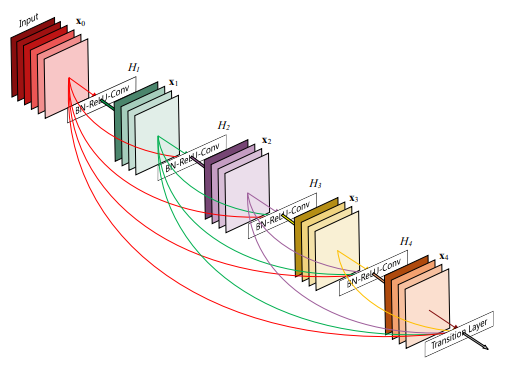
\includegraphics[width=0.7\linewidth]{figs/dense-network.png}
    \caption{Um bloco de cinco camadas de uma DenseNet. Cada camada recebe como entrada a saída de todas as camadas anteriores. Fonte: \citeonline{Huang2017}}
    \label{fig:dense-network}
\end{figure}

O componente fundamental da DenseNet é o bloco denso (ou \textit{dense block}, do inglês), que consiste em várias camadas convolucionais conectadas densamente. Cada camada dentro do bloco denso aplica três operações consecutivas: normalização em lote, seguida de uma função de ativação ReLU e, por fim, uma convolução 3×3. Após a aplicação do bloco denso, uma transição é realizada para reduzir a dimensão dos mapas de características usando uma camada de convolução 1×1, seguida por uma camada de \textit{average pooling} 2×2.

Dessa forma, a arquitetura DenseNet é composta por quatro blocos densos, cada um seguido por camadas de transição. A saída final (classificador) é obtida através de uma camada de \textit{global average pooling} e uma camada totalmente conectada com ativação \textit{softmax} para classificação. A \autoref{tab:densenet-arch} apresenta a configuração dos modelos DenseNet-121 e DenseNet-169, que são variantes da DenseNet com diferentes profundidades e que fornecem um bom equilíbrio entre complexidade e desempenho em comparação com outras arquiteturas mais profundas.

Nos últimos anos, a arquitetura DenseNet tem sido amplamente utilizada em diversas tarefas de classificação de imagens, incluindo diagnósticos médicos. Por exemplo, \cite{Rajpurkar2017} propuseram um modelo chamado CheXNet baseado na arquitetura DenseNet-121 para detectar pneumonia a partir de radiografias torácicas, superando o desempenho médio de radiologistas na métrica F1-score.

\begin{table}[!htbp]
    \centering
    \caption{Configuração dos modelos DenseNet-121 e DenseNet-169. Fonte: \citeonline{Huang2017}.}
    \footnotesize
    \begin{tabular}{|c|c|c|c|}
        \hline
        \textbf{Camadas} & \textbf{Tamanho da saída} & \textbf{DenseNet-121} & \textbf{DenseNet-169} \\
        \hline
        Convolution & 112×112 & \multicolumn{2}{c|}{7×7 conv, stride 2} \\
        \hline
        Pooling & 56×56 & \multicolumn{2}{c|}{3×3 max pool, stride 2} \\
        \hline
        Dense Block (1) & 56×56 & 
        $\left[\begin{array}{c}
        1 \times 3 \\
        3 \times 3
        \end{array}\right] \times 6$ & 
        $\left[\begin{array}{c}
        1 \times 3 \\
        3 \times 3
        \end{array}\right] \times 6$ \\
        \hline
        \multirow{2}{*}{Transition Layer (1)} & 56×56 & \multicolumn{2}{c|}{$1 \times 1$ conv} \\
        \cline{2-4}
        & 28×28 & \multicolumn{2}{c|}{$2 \times 2$ average pool, stride 2} \\
        \hline
        Dense Block (2) & 28×28 & 
        $\left[\begin{array}{c}
        1 \times 3 \\
        3 \times 3
        \end{array}\right] \times 12$ & 
        $\left[\begin{array}{c}
        1 \times 3 \\
        3 \times 3
        \end{array}\right] \times 12$ \\
        \hline
        \multirow{2}{*}{Transition Layer (2)} & 28×28 & \multicolumn{2}{c|}{$1 \times 1$ conv} \\
        \cline{2-4}
        & 14×14 & \multicolumn{2}{c|}{$2 \times 2$ average pool, stride 2} \\
        \hline
        Dense Block (3) & 14×14 & 
        $\left[\begin{array}{c}
        1 \times 3 \\
        3 \times 3
        \end{array}\right] \times 24$ & 
        $\left[\begin{array}{c}
        1 \times 3 \\
        3 \times 3
        \end{array}\right] \times 32$ \\
        \hline
        \multirow{2}{*}{Transition Layer (3)} & 14×14 & \multicolumn{2}{c|}{$1 \times 1$ conv} \\
        \cline{2-4}
        & 7×7 & \multicolumn{2}{c|}{$2 \times 2$ average pool, stride 2} \\
        \hline
        Dense Block (4) & 7×7 & 
        $\left[\begin{array}{c}
        1 \times 3 \\
        3 \times 3
        \end{array}\right] \times 16$ & 
        $\left[\begin{array}{c}
        1 \times 3 \\
        3 \times 3
        \end{array}\right] \times 32$ \\
        \hline
        \multirow{2}{*}{Classification Layer} & 1×1 & \multicolumn{2}{c|}{$7 \times 7$ global average pool} \\
        \cline{2-4}
        &  & \multicolumn{2}{c|}{1000D fully-connected, softmax} \\
        \hline
    \end{tabular}
    \label{tab:densenet-arch}
\end{table}

\subsection{Inception-v3}

A arquitetura Inception, introduzida por \citeonline{Szegedy2015} no contexto do desafio ILSVRC 2014, representou um avanço significativo na evolução das redes neurais convolucionais. Seu principal diferencial está na proposta de uma estrutura modular — o módulo Inception — que combina convoluções de diferentes tamanhos (1×1, 3×3, 5×5) e operações de \textit{pooling} em paralelo, promovendo o processamento de informações em múltiplas escalas (\autoref{inception-module}).

O GoogLeNet, uma versão da arquitetura Inception composta por 22 camadas profundas, conquistou a primeira colocação no ILSVRC 2014 \cite{Russakovsky2015}. Esse modelo destacou-se pelo excelente desempenho em tarefas de classificação e detecção de imagens, alcançado com um número de parâmetros significativamente menor em comparação a arquiteturas anteriores, como o VGG.

\begin{figure}[!htbp]
    \centering
    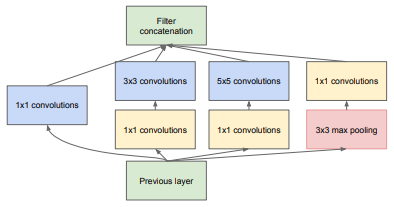
\includegraphics[width=0.7\linewidth]{figs/inception-module.png}
    \caption{Um módulo Inception. Fonte: \citeonline{Szegedy2015}}
    \label{inception-module}
\end{figure}

A arquitetura Inception-v3 \cite{Szegedy2016} representa uma evolução significativa em relação ao modelo original Inception (GoogLeNet), incorporando diversas inovações voltadas à melhoria da eficiência computacional e da acurácia. Entre as principais contribuições estão a fatoração de convoluções em operações menores e assimétricas (\autoref{inception-module-v3}), o uso mais sistemático da normalização em lote e a adoção da técnica de \textit{label smoothing} como forma de regularização. Tais aprimoramentos resultaram em um modelo mais profundo e preciso, mantendo um custo computacional viável para aplicações práticas.

\begin{figure}[!htbp]
    \centering
    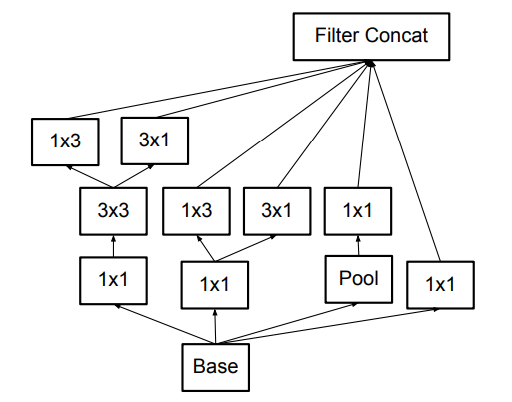
\includegraphics[width=0.5\linewidth]{figs/inception-module-v3.png}
    \caption{Um módulo Inception com fatoração de convoluções. Fonte: \citeonline{Szegedy2015}}
    \label{inception-module-v3}
\end{figure}

A \autoref{inception-v3-arch} apresenta a configuração da arquitetura Inception-v3, com um total de 42 camadas, que inclui a fatoração de convoluções tradicionais 7×7 em convoluções 3×3. A arquitetura substitui o otimizador padrão do \textit{Stochastic Gradient Descent} (SGD) por um otimizador mais avançado, o \textit{Root Mean Square Propagation} (RMSProp), favorecendo a convergência do modelo durante o treinamento, além de utilizar classificadores auxiliares com normalização em lote nas camadas intermediárias, melhorando a propagação do sinal do gradiente e, por consequência, a eficiência do treinamento.

\begin{table}[!htbp]
    \centering
    \caption{Configuração do modelo Inception-v3. Fonte \citeonline{Szegedy2016}.}
    \label{inception-v3-arch}
    \footnotesize
    \begin{tabular}{|c|c|c|c|c|}
        \hline
        \textbf{Tipo} & \textbf{Tamanho do patch/stride} & \textbf{Tamanho da entrada} \\
        \hline
        conv & $3\times3$/2 & $299\times299\times3$ \\
        \hline
        conv & $3\times3$/1 & $149\times149\times32$ \\
        \hline
        conv padded & $3\times3$/1 & $147\times147\times32$ \\
        \hline
        pool & $3\times3$/2 & $147\times147\times64$ \\
        \hline
        conv & $3\times3$/1 & $73\times73\times64$ \\
        \hline
        conv & $3\times3$/2 & $71\times71\times80$ \\
        \hline
        conv & $3\times3$/1 & $35\times35\times192$ \\
        \hline
        $3\times$Inception & - & $35\times35\times288$ \\
        \hline
        $5\times$Inception & - & $17\times17\times768$ \\
        \hline
        $2\times$Inception & - & $8\times8\times1280$ \\
        \hline
        pool & $8\times8$ & $8\times8\times2048$ \\
        \hline
        linear & logits & $1\times1\times2048$ \\
        \hline
        softmax & classifier & $1\times1\times1000$ \\
        \hline
    \end{tabular}
\end{table}

Além de seu excelente desempenho na tarefa de classificação de imagens do ILSVRC 2012 \cite{Russakovsky2015}, a arquitetura Inception-v3 tem sido utilizada em outras aplicações, incluindo o diagnóstico médico. Por exemplo, \citeonline{Mujahid2022} adotaram a arquitetura Inception-v3 para a tarefa de classificação de pneumonia em radiografias e obtiveram resultados promissores, alcançando uma acurácia de 99,29\% com um modelo \textit{ensemble}, superando outros modelos, como VGG-16 e ResNet-50.

\subsection{Aprendizado por Transferência}

O aprendizado por transferência \cite{Zhuang2021} é uma técnica de aprendizado de máquina na qual o conhecimento adquirido por um modelo treinado em uma tarefa é reutilizado para solucionar outra tarefa relacionada, mas diferente. Essa abordagem é especialmente útil para evitar o treinamento de modelos do zero, economizando tempo e recursos computacionais, além de melhorar o desempenho em tarefas com poucos dados disponíveis.

Em redes neurais, o aprendizado por transferência é frequentemente realizado reutilizando pesos de um modelo pré-treinado, cujos estágios iniciais da rede geralmente capturam características genéricas das entradas, como bordas ou texturas, que podem ser úteis para resolver novos problemas. Por exemplo, redes neurais treinadas em grandes conjuntos de dados, como o ImageNet \cite{Russakovsky2015}, podem ser reaproveitadas para resolver tarefas específicas, como a classificação de imagens médicas.

Essa estratégia é realizada através do ajuste fino (ou \textit{fine-tuning}, do inglês) do modelo pré-treinado em duas etapas principais. Na primeira, caso seja necessário, as camadas finais do modelo são substituídas por novas camadas adaptadas à tarefa-alvo, como uma camada totalmente conectada com o número de classes correspondente. Na segunda etapa, parte ou toda a rede é treinada com os novos dados. As camadas iniciais geralmente são mantidas inalteradas, enquanto as camadas finais são ajustadas para aprender as características específicas da nova tarefa.

Aplicações de visão computacional e processamento de linguagem natural têm se beneficiado da transferência de aprendizado. Ao reduzir a necessidade de grandes volumes de dados e de poder computacional, essa técnica torna-se uma alternativa viável e eficiente para o desenvolvimento de soluções baseadas em redes neurais profundas.

\section{Vision Transformer (ViT)}\label{sec:vision-transformers}

O vision transformer (ViT) é uma abordagem inovadora de aprendizado profundo que aplica a arquitetura transformer \cite{vaswani2023attentionneed}, originalmente desenvolvida para tarefas de Processamento de Linguagem Natural (PLN), ao domínio da visão computacional. Introduzido por \citeonline{Dosovitskiy2021} no artigo ``An Image is Worth 16x16 Words: Transformers for Image Recognition at Scale'', o ViT demonstrou que os transformers podem ser eficazes para tarefas de classificação de imagens ao obter excelentes resultados quando treinados em grandes conjuntos de dados (14M-300M de imagens), superando modelos tradicionais baseados em RNCs, como o ResNet.

A ideia principal do ViT, ilustrada na \autoref{fig:vision-transformer}, é tratar imagens como sequências de blocos com tamanho fixo (por exemplo, 16×16 pixels), semelhantes aos tokens em uma sequência de texto. Cada bloco é linearmente projetado em um vetor de dimensão fixa, e esses vetores resultantes são combinados em sequência junto com vetores de posição e de classe, para preservar a informação espacial e representar a classe da tarefa de classificação, respectivamente. Esses vetores são então alimentados em um modelo \textit{encoder}, onde a sequência é processada por camadas de \textit{multi-head self-attention} e \textit{feedforward}, como no transformer tradicional. O mecanismo de auto-atenção permite que o modelo aprenda relações de longo alcance entre diferentes regiões da imagem, sem a necessidade de convoluções locais, oferecendo maior flexibilidade na captura de dependências espaciais. Ao final do processamento, o token de classificação é utilizado para realizar a predição da tarefa-alvo, como prever o nível de severidade de uma doença.

Em cenários com poucos dados, as RNCs tendem a apresentar melhor desempenho, enquanto os ViTs se destacam no cenário oposto. Isso ocorre porque os transformers não possuem os vieses indutivos herdados pelas redes convolucionais, como a hierarquia espacial, a localidade e a translação equivariante, que são fundamentais para a generalização dos modelos. No entanto, modelos de ViT podem ser adaptados para funcionarem bem com conjuntos de dados reduzidos através do uso de técnicas de pré-treinamento e ajuste fino.

\begin{figure}[!htbp]
    \centering
    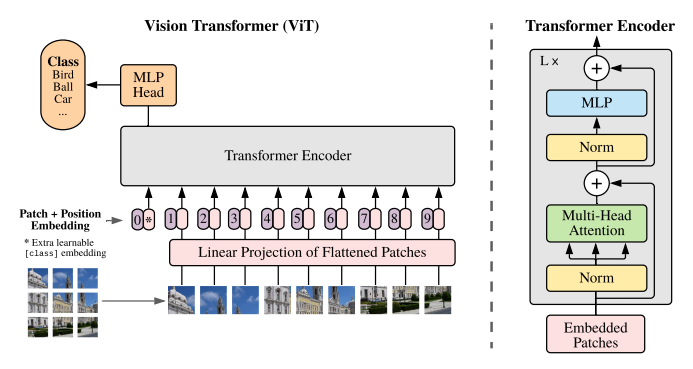
\includegraphics[width=1.0\linewidth]{figs/vision-transformer.png}
    \caption{Arquitetura do vision transformer. Fonte: \citeonline{Dosovitskiy2021}.}
    \label{fig:vision-transformer}
\end{figure}

Todas as variantes de ViT compartilham a mesma estrutura básica, que consiste na divisão da imagem em \textit{patches} de tamanho fixo, a projeção linear desses \textit{patches} em vetores de dimensão fixa, a inclusão de vetores de posição e um token de classe, e o processamento desses vetores em um \textit{encoder} de transformer. O ViT-B/16 \cite{Dosovitskiy2021} é uma das primeiras variantes da arquitetura, onde ``B'' representa o modelo base e ``16'' refere-se ao tamanho do \textit{patch} em que a imagem é dividida (16×16 pixels). Os modelos que surgiram posteriormente introduziram melhorias e adaptações buscando aumentar a eficiência e/ou reduzir a necessidade de grandes volumes de dados para treinamento. A seguir, são apresentadas as variantes que foram utilizadas nesta pesquisa.

\subsection{Data-efficient image Transformer (DeiT)}

A arquitetura DeiT, introduzida por pesquisadores do \textit{Facebook} em 2021 \cite{Touvron2021}, representa um avanço significativo na adaptação de transformers. Além de ser uma abordagem livre de convoluções, ela se destaca por não necessitar de grandes volumes de dados e infraestrutura computacional para alcançar resultados competitivos, ao contrário do que se pressupõe de arquiteturas ViT \cite{Dosovitskiy2021}.

O diferencial do DeiT reside na introdução de uma nova estratégia de distilação de conhecimento, adaptada especificamente para a arquitetura transformer. Como ilustrado na \autoref{fig:distillation-procedure}, um token de distilação é incorporado diretamente à entrada do transformer e atua de maneira similar ao token de classificação: interage com os demais tokens da rede através das camadas de auto-atenção e sua saída é observada após a última camada. Este token é treinado com o objetivo de replicar a predição de um ``modelo professor'', estratégia conhecida como \textit{hard-label distillation}:

\begin{equation}
    L_{\text{global}}^{\text{hardDistill}} = \frac{1}{2} \, L_{CE}\left( \psi(Z_s), y \right) + \frac{1}{2} \, L_{CE}\left( \psi(Z_s), y_t \right) \text{,}
\end{equation}

onde $Z_s$ são os \textit{logits} do ``modelo aluno'', $L_{CE}$ é a entropia cruzada sobre os rótulos corretos ($y$) e os rótulos preditos pelo ``modelo professor'' ($y_t = \text{argmax}_c Z_t(c)$), sendo $Z_t$ os seus \textit{logits}, e $\psi$ é a função \textit{softmax}. Como resultado, ambos os tokens compartilham informação ao longo das camadas e gradualmente convergem para vetores similares, porém ainda distintos. Por fim, seus valores são associados com classificadores lineares para produzir o rótulo da imagem.

Entre suas variantes, o modelo DeiT-B com a estratégia de distilação, que possui arquitetura semelhante ao ViT-B, é o maior modelo em termos de número de parâmetros (87 milhões). Em experimentos com o ImageNet-1K, tal modelo atingiu uma acurácia top-1 de 83,4\% (com entrada de 224×224 pixels), superando arquiteturas de RNC e inclusive variantes do ViT pré-treinadas com conjuntos de dados significativamente maiores. Adicionalmente, avaliações em tarefas de \textit{transfer learning} em diversos \textit{benchmarks} (CIFAR-10, CIFAR-100, Flowers) demonstram a capacidade de generalização do modelo, onde o DeiT ficou no mesmo nível que RNCs competitivas e superou modelos ViT tradicionais.

Diante desses resultados, o DeiT se mostra como uma alternativa promissora e eficiente aos modelos convolucionais e ViT clássicos para diversas tarefas, incluindo análise de imagens médicas. Por exemplo, \citeonline{alotaibi2022} propuseram um modelo \textit{ensemble} com ViT e DeiT (ViT-DeiT) para classificar imagens histopatológicas do câncer de mama em oito classes (benignas e malignas), obtendo um resultado de 98,17\% de acurácia.

\begin{figure}[!htbp]
    \centering
    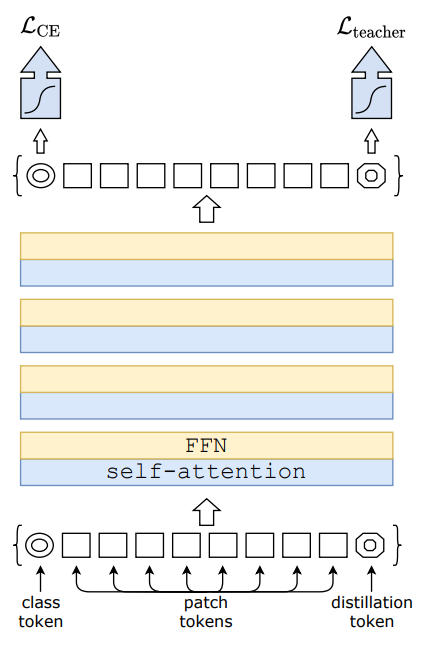
\includegraphics[width=0.5\linewidth]{figs/distillation-procedure-deit.png}
    \caption{Estratégia de distilação em transformers através da introdução de um token de distilação. Fonte: \citeonline{Touvron2021}.}
    \label{fig:distillation-procedure}
\end{figure}

\subsection{Swin Transformer}

A adaptação de arquiteturas transformer para tarefas de visão computacional apresenta desafios únicos, como a grande variação de escala das entidades visuais e a alta resolução das imagens. Em resposta a esses desafios, \citeonline{Liu2021} propuseram o Swin Transformer, uma nova arquitetura de ViT que serve como uma espinha dorsal de propósito geral para a área. O modelo introduz uma abordagem hierárquica e um mecanismo de auto-atenção baseado em janelas deslocadas, o que lhe confere eficiência e flexibilidade para modelar em múltiplas escalas com complexidade computacional linear em relação ao tamanho da imagem.

A representação hierárquica do Swin Transformer, começando com pequenos \textit{patches} e aumentando gradualmente a resolução (\autoref{fig:swin-t-vs-vit}), e o esquema de janelas deslocadas são os principais diferenciais do Swin Transformer em relação a outras arquiteturas ViT, limitando o cálculo da auto-atenção a janelas locais e não sobrepostas, ao mesmo tempo que permite conexões cruzadas entre essas janelas em camadas consecutivas. Essa estratégia aumenta significativamente o poder de modelagem sem sacrificar a eficiência.

\begin{figure}[!htbp]
    \centering
    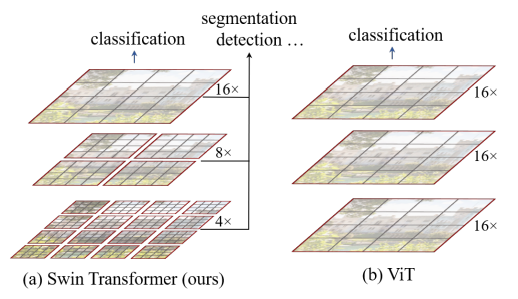
\includegraphics[width=0.7\linewidth]{figs/swin_t_vs_vit.png}
    \caption{(a) Mapa de características hierárquico do Swin Transformer. (b) Em contraste, o formato de resolução única dos mapas de características do ViT. Fonte: \citeonline{Liu2021}.}
    \label{fig:swin-t-vs-vit}
\end{figure}

A arquitetura do Swin Transformer, ilustrada na \autoref{fig:swin-t-arch}, representa a versão \textit{tiny} do modelo (Swin-T), que é a menor variante. Inicialmente, a imagem é dividida em \textit{patches} (tokens), e um conjunto de blocos Swin Transformer é aplicado sobre esses tokens. Para criar a hierarquia, camadas de fusão de \textit{patches} reduzem a resolução espacial (por um fator de 2x) e aumentam a dimensão dos canais (por 2x) à medida que a rede se aprofunda. Isso permite que o modelo gere mapas de características em múltiplas escalas (por exemplo, 4x, 8x, 16x e 32x), tornando-o compatível com tarefas de predição densa, como a detecção de objetos e a segmentação.

\begin{figure}[!htbp]
    \centering
    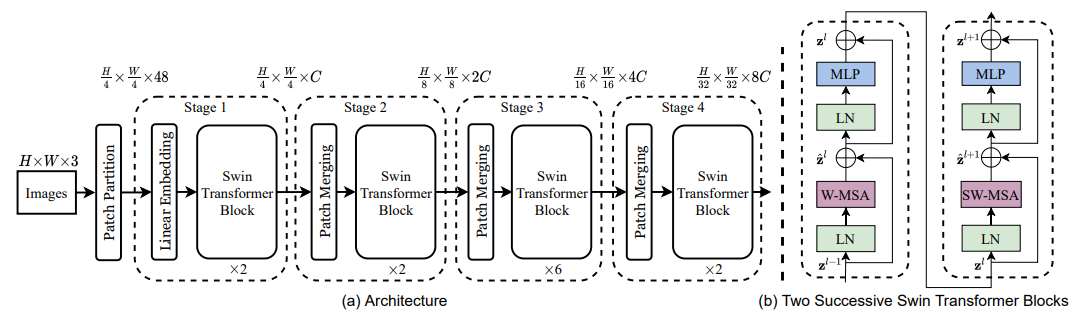
\includegraphics[width=\linewidth]{figs/swin_t-arch.png}
    \caption{(a) A arquitetura do Swin Transformer (Swin-T); (b) Dois blocos Swin Transformer sucessivos. Fonte: \citeonline{Liu2021}.}
    \label{fig:swin-t-arch}
\end{figure}

Em camadas consecutivas, os blocos Swin Transformer alternam entre duas configurações de atenção: uma baseada em janelas regulares (W-MSA) e outra em janelas deslocadas (SW-MSA). A formulação de dois blocos sucessivos é dada por:

\begin{equation}
    \hat{z}^{l} = \text{W-MSA}(\text{LN}(z^{l-1}))+z^{l-1} \text{ ,}
\end{equation}
\begin{equation}
    z^{l} = \text{MLP}(\text{LN}(\hat{z}^{l}))+\hat{z}^{l} \text{ ,}
\end{equation}
\begin{equation}
    \hat{z}^{l+1} = \text{SW-MSA}(\text{LN}(z^{l}))+z^{l} \text{ ,}
\end{equation}
\begin{equation}
    z^{l+1} = \text{MLP}(\text{LN}(\hat{z}^{l+1}))+\hat{z}^{l+1} \text{ ,}
\end{equation}

onde $\hat{z}$ e $z$ denotam as saídas dos módulos de atenção e da MLP para um bloco $l$, respectivamente. A atenção é sempre calculada com um viés de posição relativa, o que se mostrou crucial para o desempenho do modelo.

O Swin Transformer possui quatro configurações principais: Swin-T, Swin-S, Swin-B e Swin-L, que variam em capacidade. A versão base (Swin-B), possui 88 milhões de parâmetros e alcançou uma acurácia top-1 de 83,5\% no ImageNet-1K (com entrada de 224×224 pixels), superando os modelos ViT-B/16 (77,91\%) e DeiT-B com distilação (83,4\%) \cite{Dosovitskiy2021, Touvron2021}.

\subsection{Dual Attention Vision Transformers (DaViT)}

Com o avanço das arquiteturas de ViT, diversos métodos têm buscado o equilíbrio entre a capacidade de capturar contexto global e a eficiência computacional necessária para lidar com imagens de alta resolução. Nesse contexto, \citeonline{ding2022davitdualattentionvision} propuseram uma nova arquitetura de ViT que introduz um mecanismo de atenção dual, combinando janelas espaciais de atenção e grupos de canais de atenção, de forma a integrar representações locais e globais de maneira eficiente e complementar.

O principal diferencial do DaViT está na aplicação do mecanismo de atenção no domínio dos canais. Após transpor o vetor de características gerado pelo mecanismo de auto-atenção em blocos locais, cada canal passa a representar uma visão abstrata global da imagem. A atenção é então aplicada entre os grupos de canais, o que permite o modelo capturar interações globais com complexidade linear. A \autoref{fig:spatial-and-channel-window-self-attention} ilustra a perspectiva ortogonal do DaViT.

\begin{figure}[!htbp]
    \centering
    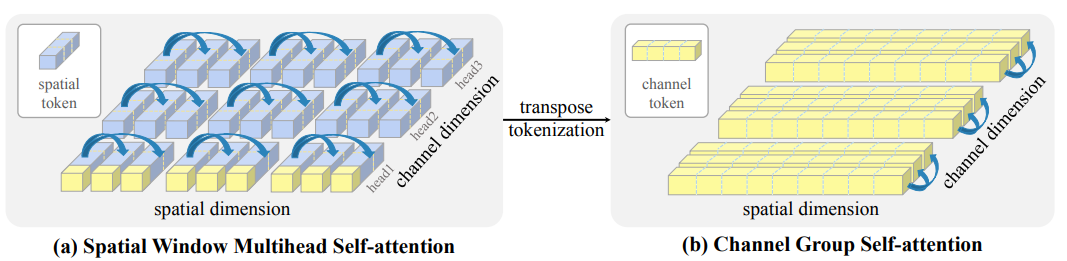
\includegraphics[width=\linewidth]{figs/spatial-and-channel-window-self-attention.png}
    \caption{(a) \textit{Spatial window multihead self-attention} divide a dimensão espacial em janelas locais, onde cada janela contém múltiplos tokens espaciais. (b) \textit{Channel group single-head self-attention} agrupa tokens de canal em múltiplos grupos. Fonte: \citeonline{ding2022davitdualattentionvision}.}
    \label{fig:spatial-and-channel-window-self-attention}
\end{figure}

O mecanismo de atenção local, aplicado em janelas espaciais, está ilustrado na \autoref{fig:davit-arch}(b). Ele divide a imagem em janelas não sobrepostas e aplica a atenção apenas entre os tokens espaciais (\textit{patches} da imagem) dentro de cada janela. Supondo $N_w$ janelas diferentes contendo $P_w$ \textit{patches} cada, onde $P=P_w * N_w$, o mecanismo de atenção local pode ser representado como:

\begin{equation}
    \text{A}_{\text{window}}(Q, K, V) = \lbrace \text{A}(Q_i,K_i,V_i) \rbrace ^{N_w}_{i=0} \text{ ,}
\end{equation}

onde $Q_i$, $K_i$ e $V_i$ são os vetores de consulta, chave e valor correspondentes a cada janela. Isso reduz significativamente o custo computacional, visto que a complexidade é linear com tamanho espacial $P$, embora isso limite a capacidade do modelo de capturar relações de longo alcance.

\begin{figure}[!htbp]
    \centering
    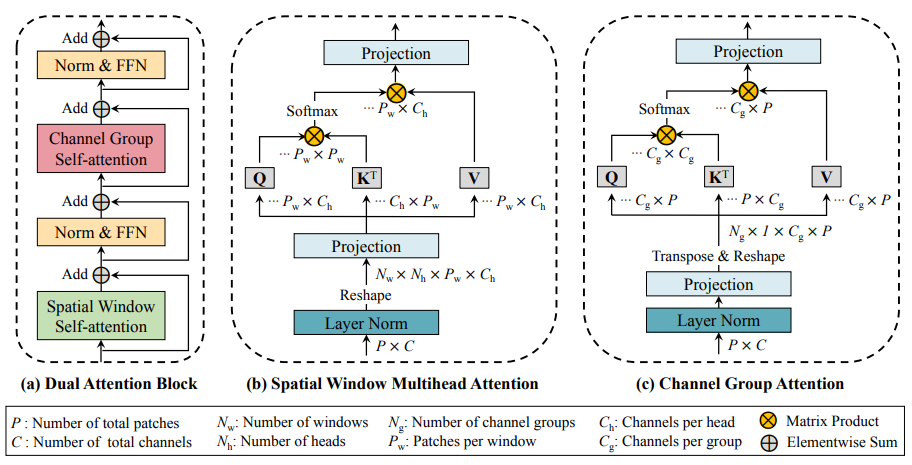
\includegraphics[width=\linewidth]{figs/davit-arch.png}
    \caption{Arquitetura DaViT do bloco \textit{dual attention}. Fonte: \citeonline{ding2022davitdualattentionvision}.}
    \label{fig:davit-arch}
\end{figure}

Já o mecanismo de atenção global, aplicado em grupos de canais, é ilustrado na \autoref{fig:davit-arch}(c). Ao invés de atuar sobre \textit{patches} espaciais, esta abordagem transpõe o vetor de características e aplica a atenção em tokens de canal. Cada token de canal representa uma visão abstrata global da imagem, pois abrange todos os locais espaciais. Ao computar a atenção entre esses tokens, o modelo consegue naturalmente capturar interações globais com complexidade linear. Formalmente, seja $N_g$ o número de grupos e $C_g$ o número de canais em cada grupo, tem-se que $C=N_g * C_g$. Assim:

\begin{equation}
    \text{A}_{\text{channel}}(Q, K, V) = \lbrace \text{A}_{\text{group}}(Q_i,K_i,V_i)^T \rbrace^{N_g}_{i=0}
\end{equation}

\begin{equation}
    \text{A}_{\text{group}}(Q_i, K_i, V_i) = \text{softmax}\left(\frac{Q_i^T K_i}{\sqrt{C_g}}\right) V_i^T \text{ ,}
\end{equation}

onde $Q_i$, $K_i$, $V_i$ $\in \mathbb{R}^{P \times C_g}$ são os vetores de consulta, chave e valor correspondentes a cada grupo de canais.

Existem três configurações diferentes da arquitetura DaViT para classificação de imagens, detecção de objetos e segmentação, que diferem na quantidade de camadas, tamanho do \textit{patch}, número de grupos em cada canal e número de cabeças de atenção. O modelo DaViT-B é a maior configuração, com quase 88 milhões de parâmetros, e obteve acurácia top-1 de 84,6\% no ImageNet-1K (com entrada de 224×224 pixels), superando modelos como o DeiT-B com distilação (83,4\%) e o Swin-B (83,5\%) \cite{Touvron2021, Liu2021}.

\subsection{Multi-Axis Vision Transformer (MaxViT)}

A escalabilidade da auto-atenção em transformers para imagens de alta resolução tem sido um desafio significativo, limitando sua aplicação em arquiteturas de visão de ponta. Para superar essa barreira, \citeonline{maxvit2022} propuseram o MaxViT, uma arquitetura que introduz um modelo de atenção eficiente e escalável, denominado auto-atenção multi-eixo (\textit{multi-axis self-attention} - Max-SA). Essa abordagem combina convoluções e um novo módulo de atenção que efetivamente captura interações espaciais locais e globais com complexidade apenas linear, permitindo que o modelo ``veja'' globalmente em todas as etapas da rede.

A \autoref{fig:max-sa} ilustra o conceito fundamental do Max-SA. O mecanismo de atenção em bloco é responsável pelas interações locais. Seja $X \in \mathbb{R}^{H \times W \times C}$ a entrada de um mapa de características, a ideia é dividi-lo em um vetor na forma $(\frac{H}{P} \times \frac{W}{P} \text{, } P \times P \times C)$, representando a partição da imagem em janelas não sobrepostas de tamanho $P \times P$. A atenção é então aplicada dentro dessas janelas, permitindo que o modelo capture relações locais.

O módulo de atenção em grade, por outro lado, é responsável pelas interações globais do espaço 2D. Em vez de usar janelas de tamanho fixo, ela divide o mapa de características em uma grade uniforme na forma ($G \times G \text{, } \frac{H}{G} \times \frac{W}{G} \text{, } C$) usando um tamanho de grade fixo $G \times G$. Isso cria janelas de tamanho adaptativo, e a auto-atenção é aplicada entre os pixels que caem na mesma posição relativa dentro de cada célula da grade. Esse processo corresponde a uma mistura espacial dilatada e global dos tokens, permitindo um campo receptivo global com complexidade também linear.

\begin{figure}[!htbp]
    \centering
    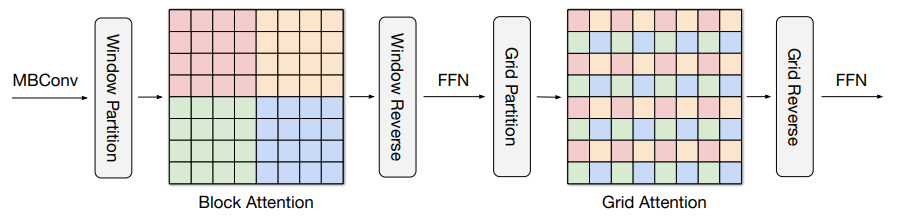
\includegraphics[width=\linewidth]{figs/max-sa.png}
    \caption{Módulo de atenção multi-eixo do MaxViT (Max-SA). O módulo \textit{block-attention} aplica atenção dentro das janelas, enquanto o módulo \textit{grid-attention} atua globalmente no espaço 2D. Fonte: \citeonline{maxvit2022}.}
    \label{fig:max-sa}
\end{figure}

Esses dois mecanismos de atenção são combinados com uma camada de convolução MBConv para formar o bloco MaxViT, a unidade fundamental da arquitetura, conforme ilustrado na \autoref{fig:maxvit-arch}. Esses blocos são empilhados para formar a arquitetura MaxViT, que por sua vez possui algumas variantes, como MaxViT-T, MaxViT-B e MaxViT-L, que aumentam em número de blocos e canais em cada estágio para escalar a capacidade do modelo. O modelo MaxViT-L, por exemplo, estabeleceu um novo estado da arte na classificação do ImageNet-1K, alcançando uma acurácia top-1 de 85,17\% (com entrada de 224×224 pixels), seguido pelo MaxViT-B com 84,95\%, superando também modelos anteriores como o DeiT-B (83,4\%), Swin-B (83,5\%) e DaViT-B (84,6\%).

\begin{figure}[!htbp]
    \centering
    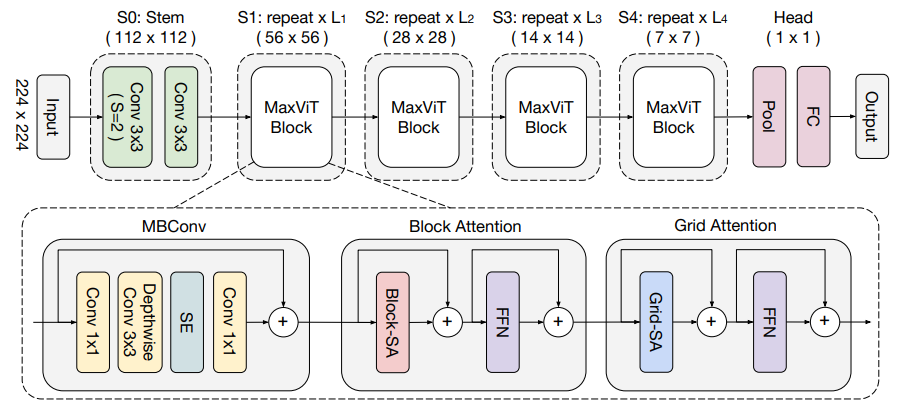
\includegraphics[width=\linewidth]{figs/maxvit-arch.png}
    \caption{Arquitetura MaxViT. Fonte: \citeonline{maxvit2022}.}
    \label{fig:maxvit-arch}
\end{figure}

\subsection{Global Context Vision Transformer (GCViT)}

Em 2022, \citeonline{gcvit2022} introduziram o GCViT, uma nova arquitetura que aumenta a eficiência de cômputo e parâmetros ao integrar módulos de auto-atenção de contexto global com a atenção local tradicional, modelando de forma eficaz as interações espaciais de curta e longa distância. Além disso, os autores propuseram o uso de blocos residuais Fused-MBConv modificados, que incorporam o viés indutivo convolucional na arquitetura.

O GCViT foi desenvolvido para superar limitações presentes em modelos ViT anteriores. Embora esses modelos tenham representado avanços importantes, o campo receptivo restrito às janelas locais limitava a captura de informações de longo alcance, e os esquemas de deslocamento de janelas cobriam apenas uma fração do contexto global.

O diferencial do GCViT é a sua capacidade de capturar informações globais sem a necessidade de operações custosas, como o deslocamento de janelas. Para isso, a cada estágio da sua arquitetura hierárquica, o modelo utiliza um gerador de consultas para extrair ``tokens de consulta globais''. Esses tokens globais, que contêm informações contextuais de diferentes regiões da imagem, são então compartilhados entre todos os módulos de atenção global para interagir com as representações locais de chave e valor. A \autoref{fig:gcvit-attention} ilustra a diferença entre a atenção local e a atenção global com consultas globais.

\begin{figure}[!htbp]
    \centering
    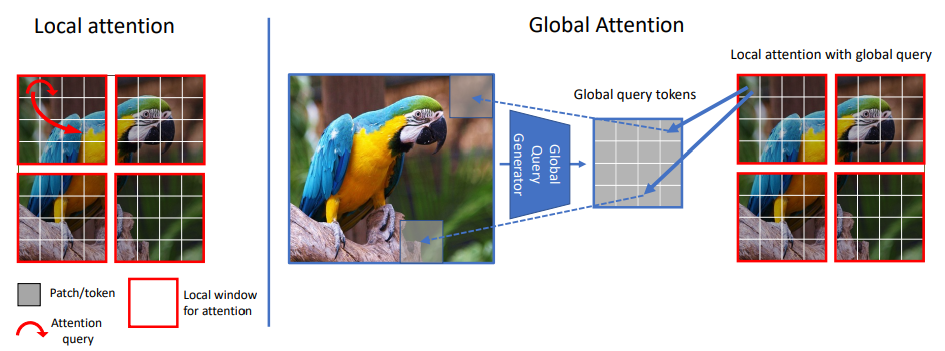
\includegraphics[width=\linewidth]{figs/gcvit-attention.png}
    \caption{Formulação da atenção no GCViT. A atenção local (esquerda) é restrita a uma janela local. Na atenção global (direita), um gerador de consultas extrai características de toda a imagem para formar tokens de consulta globais, que então interagem com os tokens de chave e valor locais, permitindo a captura de informações de longo alcance. Fonte: \citeonline{gcvit2022}.}
    \label{fig:gcvit-attention}
\end{figure}

A arquitetura geral do GCViT é apresentada na \autoref{fig:gcvit-arch}. A cada estágio, blocos de atenção local e global são aplicados de forma alternada. Enquanto a atenção local modela as informações de curto alcance, a atenção global utiliza os consultas pré-calculados pelo gerador de consultas para interagir com as representações locais de chave e valor dentro de cada janela. A atenção global é formulada como:

\begin{equation}
    \text{Attention}(q_g, k, v) = \text{Softmax}\left(\frac{q_g k}{\sqrt{d}} + b\right)v \text{ ,}
\end{equation}

onde $q_g$ são os consultas globais, $k$ e $v$ são as chaves e valores locais, $d$ é um fator de escala e $b$ é um viés de posição relativa aprendido. Adicionalmente, o GCViT incorpora blocos Fused-MBConv modificados, tanto no gerador de consultas quanto nos módulos de \textit{downsampling}, para introduzir um viés indutivo convolucional e modelar dependências entre canais.

\begin{figure}[!htbp]
    \centering
    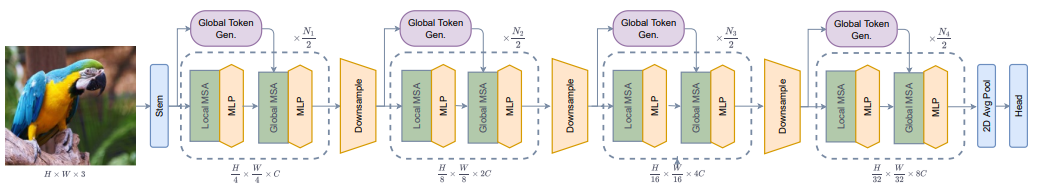
\includegraphics[width=\linewidth]{figs/gcvit-arch.png}
    \caption{Arquitetura do GCViT. A cada estágio, um gerador de tokens extrai consultas globais que interagem com as representações locais de chave e valor para capturar contexto de longo alcance. Fonte: \citeonline{gcvit2022}.}
    \label{fig:gcvit-arch}
\end{figure}

O GCViT é apresentado em diversas configurações, que variam em capacidade. Na classificação no ImageNet-1K, as variantes GCViT-S (51 milhões de parâmetros) e GCViT-B (90 milhões de parâmetros) atingiram acurácias top-1 de 84,3\% e 85,0\%, respectivamente, com resolução de 224×224 pixels e sem pré-treinamento. Esses resultados superam modelos de tamanho comparável, como o Swin-B (83,5\%) e o MaxViT-B (84,9\%).

\section{Funções de Perda} \label{sec:funcoes-perda}

A função de perda é um componente essencial no treinamento de modelos, pois guia o ajuste dos pesos da rede neural ao quantificar a diferença entre as previsões e os rótulos reais. Neste trabalho, foram utilizadas duas funções de perda com o objetivo de compará-las: a entropia cruzada (ou \textit{cross-entropy}, do inglês) e a \textit{Conditional Ordinal Regression for Neural Networks} (CORN).

\subsection{Entropia Cruzada}

A entropia cruzada é uma opção comum para problemas de classificação, pois mede o quão bem as previsões do modelo se alinham com os rótulos reais. Ela é definida como:

\begin{equation}
    J(\Theta) = -\frac{1}{m} \sum_{i=1}^{m} \sum_{k=1}^{K} y_{k}^{(i)} \log(\hat{p}_k^{(i)}) \text{,}
\end{equation}

onde $y_{k}^{(i)}$ é a probabilidade real da classe $k$ para o exemplo $i$.

Ao penalizar mais fortemente casos em que o modelo apresenta baixa confiança na classe correta, a entropia cruzada, de modo geral, contribui para aumentar a precisão do modelo para tarefas de classificação. No entanto, ela não leva em consideração a natureza ordinal das classes, o que constitui uma limitação em problemas onde a ordem das classes é relevante, como no problema abordado neste trabalho.

\subsection{Conditional Ordinal Regression for Neural Networks (CORN)}

\citeonline{Shi_2023} propuseram um framework de regressão ordinal para redes neurais profundas, chamado CORN, que é projetado para lidar com tarefas de classificação ordinal, mantendo a consistência ordinal entre as classes. Dado um problema de classificação com $K$ classes e um conjunto de treino $D = \{(x^{[i]}, y^{[i]})\}_{i=1}^{N}$, onde $x^{[i]}$ é a entrada e $y^{[i]}$ é o rótulo ordinal, o CORN divide o problema de classificação ordinal em $K-1$ tarefas de classificação binária associadas às classes $r_1$, $r_2$, $...$, $r_K$, onde $y_{k}^{[i]} \in \lbrace 0 \text{,} 1 \rbrace$ indica se o exemplo $y^{[i]}$ excede a classe $r_k$ ou não (\autoref{fig:corn-nn}).

A saída da $k$-ésima tarefa binária $f_k (x^{[i]})$ representa a probabilidade condicional de que o exemplo $x^{[i]}$ exceda a classe $r_k$, e é calculada como:

\begin{equation}
    f_k (x^{[i]}) = \hat{P} (y^{[i]} > r_k | y^{[i]} > r_{k-1}) \text{,}
\end{equation}

onde os eventos estão aninhados: $\lbrace y^{[i]} > r_k \rbrace \subseteq \lbrace y^{[i]} > r_{k-1} \rbrace$.

\begin{figure}[!htbp]
    \centering
    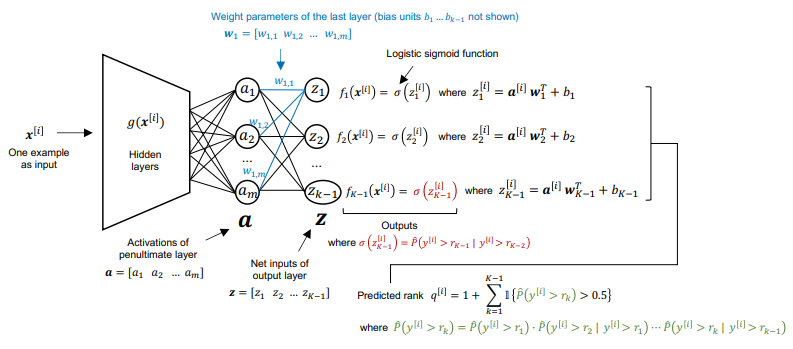
\includegraphics[width=\linewidth]{figs/corn-nn.png}
    \caption{Arquitetura do framework CORN. Fonte: \citeonline{Shi_2023}.}
    \label{fig:corn-nn}
\end{figure}

Com o objetivo de estimar $f_1 (x^{[i]})$ e as probabilidades condicionais $f_2 (x^{[i]})$, ..., $f_{K-1} (x^{[i]})$, o modelo CORN utiliza uma rede neural com $K-1$ saídas, onde cada saída é treinada para prever a probabilidade de que o rótulo ordinal exceda a classe correspondente. Para isso, são construídos subconjuntos de treino condicionais da seguinte maneira:

\begin{equation}
    \begin{split}
        &S_1: \text{todo } \lbrace (x^{[i]}, y^{[i]}) \rbrace \text{, para } i \in \lbrace 1,...,N \rbrace \text{,}\\
        &S_2: \lbrace (x^{[i]}, y^{[i]}) | y^{[i]} > r_1 \rbrace \text{,}\\
        &...\\
        &S_{K-1}: \lbrace (x^{[i]}, y^{[i]}) | y^{[i]} > r_{k-2} \rbrace \text{,}
    \end{split}
\end{equation}

onde $N = |S_1| \ge |S_2| \geq |S_3| \geq ... \geq |S_{K-1}|$, e $|S_k|$ é o número de exemplos no subconjunto $S_k$.

Para treinar o modelo CORN, seja $f_j (x^{[i]})$ o valor predito pela rede neural para o $j$-ésimo nó da camada de saída, a função de perda a ser minimizada é definida como:

\begin{equation}
    \begin{split}
        L(X,y) = -\frac{1}{\sum_{j=1}^{K-1} |S_j|} \sum_{j=1}^{K-1} \sum_{i=1}^{|S_j|} [\text{log}(f_j (x^{[i]})) \cdot \mathbb{I}(y^{[i]} > r_j) \\
        +\text{log}(1 - f_j (x^{[i]})) \cdot \mathbb{I}(y^{[i]} \leq r_j)] \text{,}
    \end{split}
\end{equation}

onde $\mathbb{I}(\cdot)$ é a função indicadora, que retorna 1 se a condição for verdadeira e 0 caso contrário. Essa função de perda penaliza as previsões incorretas de forma proporcional à distância ordinal entre as classes, permitindo que o modelo aprenda a estrutura ordinal dos rótulos. Por fim, para obter o índice da classe predita $q$ do $i$-ésimo exemplo, basta calcular:

\begin{equation}
    q^{[i]} = 1 + \sum_{j=1}^{K-1} \mathbb{I}(\hat{P}(y^{[i]} > r_j) > 0.5) \text{,}
\end{equation}

onde a classe predita será $r_{q^{[i]}}$.

\section{Avaliação e métricas de desempenho} \label{sec:avaliacao-metricas}

Para avaliar o desempenho dos modelos na tarefa de classificação da severidade da OA de joelho, foram empregadas métricas amplamente utilizadas, como acurácia, precisão, revocação, F1-score e \textit{Quadratic Weighted Kappa} (QWK). A matriz de confusão foi utilizada para visualizar a distribuição das previsões corretas e incorretas entre as diferentes classes, enquanto a métrica AUC-ROC (Área Sob a Curva da Característica de Operação do Receptor) avaliou a capacidade do modelo de distinguir uma classe em relação às demais. Essas métricas fornecem uma visão abrangente do desempenho dos modelos. Para o cálculo delas, foram adotados os seguintes acrônimos nas respectivas fórmulas:

\begin{itemize}
    \item $TP$ é o número de verdadeiros positivos,
    \item $TN$ é o número de verdadeiros negativos,
    \item $FP$ é o número de falsos positivos,
    \item $FN$ é o número de falsos negativos.
\end{itemize}

\subsection{Acurácia}
A acurácia mede a proporção de previsões corretas em relação ao total de exemplos. Ela pode ser calculada pela fórmula:

\begin{equation}
    \text{Acurácia} = \frac{TP + TN}{TP + TN + FP + FN}
\end{equation}

\subsection{Precisão}
A precisão indica a proporção de exemplos classificados como positivos que realmente são positivos. Ela é calculada pela fórmula:

\begin{equation}
    \text{Precisão} = \frac{TP}{TP + FP}
\end{equation}

\subsection{Revocação}
A revocação (ou \textit{recall}, do inglês) mede a capacidade do modelo de identificar corretamente todos os exemplos positivos. É definida como:

\begin{equation}
    \text{Revocação} = \frac{TP}{TP + FN}
\end{equation}

\subsection{F1-Score}
O F1-score é a média harmônica entre a precisão e a revocação, e é uma métrica útil quando busca-se um equilíbrio entre os dois. A fórmula do F1-score é:

\begin{equation}
    F1 = 2 \cdot \frac{\text{Precisão} \cdot \text{Revocação}}{\text{Precisão} + \text{Revocação}}
\end{equation}

\subsection{Quadratic Weighted Kappa (QWK)}
O QWK é uma métrica que avalia a concordância entre as previsões do modelo e os rótulos reais, levando em consideração a característica ordinal das classes. É especialmente útil para este estudo devido à natureza ordinal das classes de severidade da OA de joelho, onde erros maiores são mais penalizados do que erros menores. O QWK é calculado pela seguinte fórmula:

\begin{equation}
    QWK = 1 - \frac{\sum_{i,j} w_{ij} O_{ij}}{\sum_{i,j} w_{ij} E_{ij}} \text{,}
\end{equation}

onde $w_{ij}$ é a matriz de pesos que penaliza os erros de classificação, $O_{ij}$ é a matriz de confusão observada e $E_{ij}$ é a matriz de confusão esperada. O QWK varia entre -1 e 1, onde 1 indica concordância perfeita, 0 indica concordância aleatória e valores negativos indicam discordância.

\subsection{Matriz de Confusão}
A matriz de confusão é uma ferramenta para visualizar o desempenho do modelo de classificação, detalhando as previsões corretas e incorretas em cada classe. Ela apresenta os valores de $TP$, $TN$, $FP$ e $FN$ de forma estruturada, permitindo avaliar o desempenho em classes específicas.

\[
\begin{array}{|c|c|c|}
\hline
 & \text{Previsto Positivo} & \text{Previsto Negativo} \\
\hline
\text{Verdadeiro Positivo} & TP & FN \\
\hline
\text{Verdadeiro Negativo} & FP & TN \\
\hline
\end{array}
\]

\subsection{AUC-ROC}
A métrica AUC-ROC (Área Sob a Curva da Característica de Operação do Receptor) é bastante útil, pois mede a capacidade do modelo de separar as classes positivas e negativas. A curva ROC é um gráfico que exibe a taxa de verdadeiros positivos (sensibilidade) em função da taxa de falsos positivos. A AUC, por sua vez, quantifica a área sob essa curva, variando de 0 a 1, onde 0,5 representa um modelo aleatório e 1 representa um modelo perfeito. A AUC-ROC é calculada pela seguinte integral:

\begin{equation}
    \text{AUC-ROC} = \int_{0}^{1} \text{TPR}(FPR) \text{ d}FPR \text{,}
\end{equation}

onde $TPR$ é a taxa de verdadeiros positivos e $FPR$ é a taxa de falsos positivos.

\subsection{Eficiência computacional}

Além da performance em termos de métricas relacionadas à classificação, a eficiência computacional constitui um aspecto fundamental na avaliação de modelos de aprendizado profundo, especialmente em contextos com restrições de tempo ou recursos computacionais. Essa métrica torna-se ainda mais relevante quando se considera a aplicabilidade clínica dos modelos, onde a rapidez na inferência pode ser crucial para a tomada de decisão em tempo real.

Para mensurar a eficiência computacional, foram considerados três aspectos principais: o tempo de treinamento, o tempo de inferência e a quantidade de operações computacionais realizadas por cada modelo. Os tempos de treinamento e inferência foram calculados por meio da diferença entre os instantes de término e início de cada processo:

\begin{equation}
    \text{Tempo Total} = \text{Tempo Final} - \text{Tempo Inicial} \text{.}
\end{equation}

A terceira métrica adotada foi a quantidade estimada de operações de ponto flutuante, conhecida como \textit{Floating Point Operations} (FLOPs), uma medida amplamente utilizada para quantificar o custo computacional associado à execução de modelos de redes neurais. A quantidade de FLOPs está diretamente relacionada à complexidade arquitetural do modelo, abrangendo as operações realizadas durante as fases de \textit{forward} e \textit{backward}, bem como o número de amostras e épocas de treinamento \cite{Lohn2022}.

\subsection{Predição Conformal} \label{sec:conformal-prediction}

A predição conformal é uma técnica estatística que fornece intervalos de confiança às previsões de qualquer modelo de aprendizado de máquina. Dada uma probabilidade de erro $\epsilon$, o método gera, para cada nova entrada, um conjunto de possíveis rótulos que inclui a predição $\hat{y}$ do modelo, com garantia teórica de que o rótulo verdadeiro estará nesse conjunto com probabilidade de ao menos $1 - \epsilon$ \cite{angelopoulos2021gentle}.

Considere um modelo classificador $\hat{f}$ e um conjunto de imagens classificadas em uma das $K$ classes possíveis. Para cada imagem $x$, o modelo atribui uma distribuição de probabilidades $\hat{f}(x) \in [0,1]^K$ sobre as classes, geralmente obtida por meio da função \textit{softmax}. Com base nessas probabilidades, utiliza-se um conjunto de calibração para então encontrar o conjunto de predição. Em resumo, a predição conformal é realizada da seguinte forma:

\begin{enumerate}
    \item Para cada par de imagem ($x$, $y$) do conjunto de calibração, calcula-se a pontuação de conformidade $s(x,y)$:
    \begin{equation}
        s(x,y) = \sum_{j=1}^{k} \hat{f}(x)_{\pi_j(x)}\text{, onde } y = \pi_k(x)
    \end{equation}
    e $\pi(x)$ é uma permutação dos rótulos de classe $\lbrace 1 \text{,...,} K \rbrace$, ordenada de acordo com a probabilidade atribuída pelo modelo, ou seja, $\hat{f}(x)_{\pi_1(x)} \geq \hat{f}(x)_{\pi_2(x)} \geq ... \geq \hat{f}(x)_{\pi_k(x)}$. Em outras palavras, as probabilidades de cada classe são somadas até que se alcance a classe correta $y$.

    \item Define-se o limiar de confiança $\hat{q}$ como sendo o quantil ${\lceil (n+1)(1-\epsilon) \rceil}/n$ sobre $s_1, ... s_n$, onde $\lceil \cdot \rceil$ é a função teto.
    \item Para um novo par de imagem de teste ($x_{\text{test}}$, $y_{\text{test}}$), forma-se o conjunto de predição $\lbrace y:s(x_{\text{test}},y_{\text{test}}) \leq \hat{q} \rbrace$:
    \begin{equation}
        C(x_{\text{test}}) = \lbrace \pi_1(x) \text{,...,} \pi_k(x) \rbrace \text{, onde } k = \sup \Bigg\lbrace k' : \sum_{j=1}^{k'} \hat{f}(x_{\text{test}})_{\pi_j(x_{\text{test}})} < \hat{q} \Bigg\rbrace + 1
    \end{equation}
\end{enumerate}

A predição conformal tem sido aplicada em diversas áreas, incluindo ciência forense, biometria e medicina, onde o objetivo é fornecer previsões mais confiáveis sobre a saída do modelo \cite{Fontana2023}. Por exemplo, \citeonline{Pereira2020} utilizaram a predição conformal para prever o intervalo de confiança da probabilidade de que pacientes com comprometimento cognitivo leve evoluam para demência.

\subsubsection{Verificação de corretude}

A verificação de corretude é uma técnica para testar se a predição conformal atende às garantias teóricas de cobertura, definida pelo \autoref{theorem:conformal-prediction}. A ideia é verificar se o conjunto de predição $C(x)$ contém o rótulo verdadeiro $y$ com probabilidade de pelo menos $1 - \epsilon$.

\begin{theorem}
\label{theorem:conformal-prediction}
    (Garantia de cobertura conformal; \citeonline{Vovk1999}) Suponha $(X_i,Y_i)_{i=1,...,n}$ e $(X_\text{test},Y_\text{test})$ são independentes e identicamente distribuídos ($i.i.d.$) e defina $\hat{q}$ como o quantil ${\lceil (n+1)(1-\epsilon) \rceil}/n$ e $C(X_\text{test}) = \lbrace y : s(X_\text{test},y) \leq \hat{q} \rbrace$. Então, segue que:

    \begin{equation}
        P(Y_\text{test} \in C(X_\text{test})) \geq 1 - \epsilon.
    \end{equation}
\end{theorem}

Para calcular a cobertura $C$, é necessário executar o algoritmo de predição conformal em um conjunto de teste. A cobertura é então calculada como a proporção de casos em que o rótulo verdadeiro $Y_\text{test}$ está contido no conjunto de predição $C(X_\text{test})$:

\begin{equation}
    C = \frac{1}{N} \sum_{i=1}^{N} \mathbb{I}(Y_i \in C(X_i)) \text{,}
\end{equation}

onde $N$ é o número de casos no conjunto de teste e $\mathbb{I}$ é a função indicadora, que retorna 1 se a condição for verdadeira e 0 caso contrário. A cobertura deve ser comparada com o nível de confiança $\epsilon$ para verificar se a predição conformal atende às garantias teóricas.

\subsection{Método de visualização}

A visualização é uma técnica importante para avaliar quais foram as regiões da imagens que ajudaram o modelo a fazer determinada previsão. O método de visualização \textit{Gradient-weighted Class Activation Mapping} (Grad-CAM) é uma técnica usada para interpretar e visualizar as decisões feitas por RNCs e ViTs. Em tarefas de classificação, como a avaliação da severidade da OA de joelho, entender quais regiões da radiografia contribuíram para a decisão do modelo é crucial para a validação e a confiança nos resultados do modelo.

O Grad-CAM fornece mapas de ativação que mostram quais partes da imagem foram mais influentes para a predição de uma classe específica \cite{Selvaraju2016}. Para isso, essa técnica utiliza os gradientes da saída da camada final da rede em relação às ativações das camadas intermediárias para gerar uma visualização da importância das regiões da imagem.

Primeiro, é gerado um mapa de localização a partir da rede para classificar a imagem usando a técnica do \textit{Class Activation Mapping} (CAM). O CAM utiliza mapas de características convolucionais, que são globalmente agrupados usando a técnica de \textit{Global Average Pooling} (GAP) e transformados linearmente para produzir uma pontuação \( y_c \) para cada classe \( c \). Especificamente, se a penúltima camada da rede produz \( K \) mapas de características \( A_k \in \mathbb{R}^{u \times v} \), esses mapas são agrupados espacialmente e combinados linearmente para gerar a pontuação:

\[
y_c = \sum_k w_{ck} \frac{1}{Z} \sum_i \sum_j A_{k_{ij}}
\]

Para produzir o mapa de localização \( L_c^{CAM} \) para a classe \( c \), a CAM calcula a combinação linear dos mapas de características finais usando os pesos aprendidos da camada final:

\[
L_c^{CAM} = \sum_k w_{ck} A_k
\]

Este mapa é então normalizado para o intervalo entre 0 e 1 para fins de visualização.

Em seguida, os gradientes são então globalmente averiguados (\textit{pooling}) para obter pesos que indicam a importância de cada canal de ativação. Esses pesos são usados para ponderar as ativações da camada convolucional final. A seguinte fórmula representa este cálculo dos pesos:

\[
\alpha_{k}^{c} = \frac{1}{Z} \sum_i \sum_j \frac{\partial y^{c}}{\partial A_{ij}^{k}}
\]

O peso \( \alpha_{k}^{c} \) representa a linearização parcial da rede e captura a importância de \(k \) para a classe \(c \). Por fim, o mapa de ativação é obtido ao multiplicar as ativações ponderadas pelos pesos dos gradientes. Esse mapa é então normalizado e sobreposto na imagem original para mostrar as áreas mais influentes na decisão do modelo.

A fórmula para o Grad-CAM pode ser expressa como:

\[
\text{Grad-CAM} = \text{ReLU} \left( \sum_{k} \alpha_{k}^{c} A^{k} \right)
\]